\documentclass[conference]{IEEEtran}
\IEEEoverridecommandlockouts
% The preceding line is only needed to identify funding in the first footnote. If that is unneeded, please comment it out.
\usepackage{cite}
\usepackage{enumitem}
\usepackage{amsmath,amssymb,amsfonts}
\usepackage{graphicx}
\usepackage{textcomp}
\providecommand{\cbrak}[1]{\ensuremath{\left\{#1\right\}}}
\providecommand{\brak}[1]{\ensuremath{\left(#1\right)}}
\usepackage{xcolor}
\def\BibTeX{{\rm B\kern-.05em{\sc i\kern-.025em b}\kern-.08em
    T\kern-.1667em\lower.7ex\hbox{E}\kern-.125emX}}
\title{
\vspace{1cm}
{\includegraphics[width=0.15\textwidth]{/storage/emulated/0/Screenshot_2024_1018_113636.jpg} \\ ESP32 Assignment} }
\author{Shaik Mohisena Tabassum \\ Roll No: FWC22279 \\ shaikmohisena123@gmail.com}
 \begin{document}
\maketitle
 \section {ABSTRACT}
 The information bit sequence 
$ \cbrak{111010101}$
 is to be transmitted by encoding with Cyclic Redundancy Check $4 \brak{CRC-4}$ code, for which the generator polynomial is $ C(x) = x^4 + x + 1$. The encoded sequence of bits is to be displayed.
\section{COMPONENTS}
The required components list is given in Table: I. The pin diagram of LCD $16\,x\,2$ is shown in Fig.1.
\begin{figure}[h]
\centering
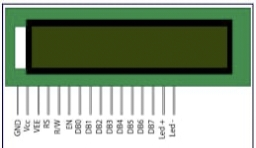
\includegraphics[width=0.35\textwidth]{/storage/emulated/0/internship/IMG_20241028_120712.jpg}
\caption{\label{fig:Gates}}
\end{figure}
 \begin{table} [htbp]
\centering
\begin{tabular}{| c | c | c |} \hline
Components & Value & Quantity \\\hline
	Vaman &  & 1 \\ \hline
	LCD &  & 1 \\ \hline
Jumper Wires &  & 15 \\ \hline
Cable & B & 1 \\ \hline
Breadboard & & 1 \\ 
\hline
\end{tabular}
\vspace{0.1cm}
\caption{\label{tab:widgets}}
\end{table}
\section{PROCEDURE}
 \begin {enumerate}
 \item
 Make the connections between Vaman and LCD as per the Table: II.
 \begin{table}[htbp]                                       
\centering                                                          
\begin{tabular}{| c | c |} \hline                                
	\textbf{Vaman} & \textbf{LCD}  \\\hline 
GPIO.19 & 4  \\ \hline        
GPIO.23 &  6 \\ \hline        
GPIO.18 & DB4 \\ \hline                                           
GPIO.17  & DB5 \\ \hline 
GPIO.16 & DB6 \\ \hline
GPIO.15 & DB7 \\ \hline
gnd  & 1,3,5,16 \\ \hline                                    
5V & 2,15 \\ \hline               
\end{tabular}                     
\vspace{0.1cm}                    
\caption{\label{tab:widgets}}     
\end{table}
\item Insert the code in the designated folder and the do the pio run
\item Now, change the credentials of the wifi given to the vaman.
\item Check the IP address of the Vaman and use the instruction as"pio run -t nobuild -t upload --upload-port 192.168.66.131" to upload the code using OTA via B-type cable connected to the phone and vaman board.
\item If connected properly, then the desired output is observed in the LCD. Otherwise, do the process again.
	\end {enumerate}
\section{RESULTS}
Download the code given in the link below and execute them to see the output as shown in Fig.2 by the LCD. 
\\ https://github.com/Tabassum4930/FWC-1/blob/main/ESP\_32/code.cpp
\begin{figure}[h] 
	\centering 
	\includegraphics[width=0.35\textwidth]{/storage/emulated/0/internship/IMG_20241028_105512_334.jpg}
	\caption{\label{fig:Gates}}    
\end{figure}
\section{CONCLUSION}
Therefore, the LCD has displayed the required output sequence using the Vaman board.
\end{document}
